\documentclass[border=6pt,tikz]{standalone}
\usepackage{tikz}
\usetikzlibrary{positioning,arrows.meta,shadows.blur}
\usepackage{amsmath,amssymb}

\definecolor{cIn}{RGB}{222,235,247}
\definecolor{cT1}{RGB}{198,224,180}
\definecolor{cT2}{RGB}{255,230,184}
\definecolor{cT3}{RGB}{248,203,203}
\definecolor{cTwin}{RGB}{217,204,236}
\definecolor{cOut}{RGB}{197,224,224}
\definecolor{cAudit}{RGB}{255,242,153}
\definecolor{cEdge}{RGB}{60,60,60}

\tikzset{
  stage/.style={
    rectangle, rounded corners=2.5pt, draw=cEdge, line width=0.9pt,
    blur shadow={shadow blur steps=4, shadow xshift=0.6pt, shadow yshift=-0.6pt},
    align=center, text=cEdge, font=\small, inner sep=2.0mm,
  },
  stageT/.style={stage, font=\small\bfseries},
  lab/.style={font=\scriptsize\itshape, text=cEdge!85},
  arr/.style={-{Stealth[length=2.8mm]}, line width=1.0pt, draw=cEdge},
}

\begin{document}
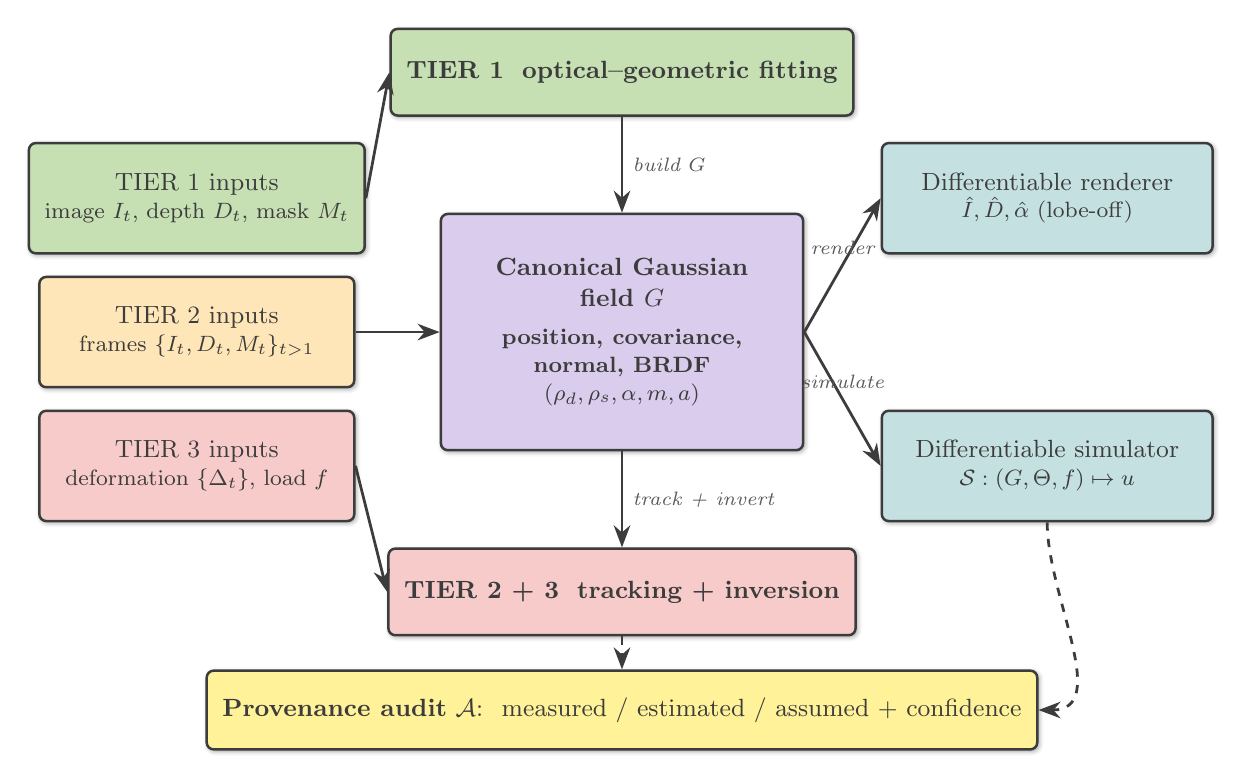
\begin{tikzpicture}

% ===== grid coordinates =====
\def\colL{0}      % left column x
\def\colC{5.4}    % center x
\def\colR{10.8}   % right column x
\def\rowT{3.4}    % top row y
\def\rowM{1.7}    % middle row y
\def\rowB{0.0}    % bottom row y

% ===== center: canonical field =====
\node[stageT, fill=cTwin, minimum width=46mm, minimum height=30mm]
  (field) at (\colC,\rowM)
  {Canonical Gaussian\\ field $G$\\[3pt]
   \footnotesize position, covariance,\\[-1pt]
   \footnotesize normal, BRDF\\[-1pt]
   \footnotesize $(\rho_d,\rho_s,\alpha,m,a)$};

% ===== left column: tier inputs =====
\node[stage, fill=cT1, minimum width=40mm, minimum height=14mm]
  (in1) at (\colL,\rowT)
  {TIER 1 inputs\\[-1pt]\footnotesize image $I_t$, depth $D_t$, mask $M_t$};
\node[stage, fill=cT2, minimum width=40mm, minimum height=14mm]
  (in2) at (\colL,\rowM)
  {TIER 2 inputs\\[-1pt]\footnotesize frames $\{I_t,D_t,M_t\}_{t>1}$};
\node[stage, fill=cT3, minimum width=40mm, minimum height=14mm]
  (in3) at (\colL,\rowB)
  {TIER 3 inputs\\[-1pt]\footnotesize deformation $\{\Delta_t\}$, load $f$};

% ===== right column: outputs =====
\node[stage, fill=cOut, minimum width=42mm, minimum height=14mm]
  (out1) at (\colR,\rowT)
  {Differentiable renderer\\[-1pt]\footnotesize $\hat{I},\hat{D},\hat{\alpha}$ (lobe-off)};
\node[stage, fill=cOut, minimum width=42mm, minimum height=14mm]
  (out2) at (\colR,\rowB)
  {Differentiable simulator\\[-1pt]\footnotesize $\mathcal{S}:(G,\Theta,f)\mapsto u$};

% ===== tier modules (top / bottom center) =====
\node[stageT, fill=cT1, minimum width=44mm, minimum height=11mm]
  (m1) at (\colC,\rowT+1.6)
  {TIER 1\; optical--geometric fitting};
\node[stageT, fill=cT3, minimum width=44mm, minimum height=11mm]
  (m23) at (\colC,\rowB-1.6)
  {TIER 2 + 3\; tracking + inversion};

% ===== audit bar (bottom) =====
\node[stage, fill=cAudit, minimum width=88mm, minimum height=10mm]
  (audit) at (\colC,\rowB-3.1)
  {\textbf{Provenance audit} $\mathcal{A}$:\; measured / estimated / assumed + confidence};

% ===== arrows: inputs -> field/modules =====
\draw[arr] (in1.east) -- (m1.west);
\draw[arr] (in2.east) -- (field.west);
\draw[arr] (in3.east) -- (m23.west);

% modules <-> field
\draw[arr] (m1.south) -- node[lab, right]{build $G$} (field.north);
\draw[arr] (field.south) -- node[lab, right]{track + invert} (m23.north);

% field -> outputs
\draw[arr] (field.east) -- node[lab, above]{render} (out1.west);
\draw[arr] (field.east) -- node[lab, above]{simulate} (out2.west);

% audit connections
\draw[arr, dashed] (m23.south) -- (audit.north);
\draw[arr, dashed] (out2.south) to[out=-90,in=0] (audit.east);

\end{tikzpicture}
\end{document}
